\documentclass[11pt]{article}
\usepackage[margin=1in]{geometry}
\usepackage{amsmath,amssymb,graphicx,longtable,booktabs,natbib,url,needspace}
\usepackage[hidelinks]{hyperref}
\setlength{\emergencystretch}{3em}
\setlength{\tabcolsep}{3pt}
\title{MarketPulse: Retrospective Evidence on Forecast Complexity, Temporal Robustness, and Delayed Uncertainty Calibration}
\author{Yug More\\\texttt{yugmore20@gmail.com}}
\date{October 2026 --- research manuscript draft}
\begin{document}
\maketitle

Research manuscript draft, October 2026. This work originated in a collaborative course project. Current affiliations, final authorship, contribution statements and consent must be confirmed before submission. This document is not a peer-reviewed publication.

\section*{Abstract}

We investigate whether greater model complexity yields reliable improvements in financial return forecasting under a common chronological evaluation protocol. Two repository price-index histories support 282 expanding-window folds and 355320 out-of-sample model forecasts at horizons of 1, 5 and 20 sessions. Zero return, a frozen training-target mean, standardized linear regression, random forest and a one-layer sequence LSTM are evaluated on shared origins. Random forest has the smallest native pooled RMSE in three index/horizon cells, but no random-forest improvement over either simple baseline survives the original 18-comparison Holm family. The LSTM has the largest pooled RMSE in all six native cells. Expanded five-seed sensitivity covers 30 selected folds rather than the full history; no ML improvement over either baseline survives its separate 30-comparison family, and NASDAQ-100 long-horizon LSTM ranks still range from first to fifth. Four bounded, delayed-feedback adaptive interval variants are evaluated retrospectively. The designated variant has 20 adjusted interval-score improvements within a 60-comparison family, confined to S\&P 500 short horizons, while long-horizon undercoverage and 1494 nominal-level nesting violations persist. Historical rehearsals are not independent confirmation. These results support a qualified comparison of the tested procedures, not universal model inferiority, unseen-market generalization, distribution-free coverage or economic profitability. [C01,C02,C08,C09,C12,C15,C19,C24,C35,C36]

\section*{1. Introduction and motivation}

Forecast accuracy, stability across periods, and the reliability of uncertainty estimates are distinct empirical questions. A flexible model can fit a training history without improving on a simple forecast on later observations. Likewise, a low average error or apparently close nominal coverage can conceal an unfavorable market regime, optimizer realization or forecast horizon. MarketPulse addresses these distinctions through a common return target and comparable evaluation samples, rather than treating model complexity as evidence of usefulness.

The project began with course notebooks whose targets, samples and stored outputs were not directly comparable. The canonical study is a subsequent shared-target experiment. Earlier notebooks and terminal-window scores remain historical context; they are not additional independent replications of the walk-forward findings. The repository preserves the original materials and the recovery record. [E:history]

All performance findings in this paper are retrospective. Model families and histories had already been examined before follow-up statistical and calibration analyses. Freezing a follow-up configuration before its execution does not make the underlying data untouched. No prospective or independent chronological validation outcome is available. [C04,E:protocols]

\section*{2. Research questions and contributions}

RQ1 asks whether random forest or the canonical LSTM improves return errors consistently over zero and historical-mean forecasts. RQ2 asks how rankings depend on horizon, native versus common-calendar evaluation, selected periods and random seeds. RQ3 asks whether fixed or delayed adaptive intervals improve coverage and proper scores without hiding width or nesting failures. RQ4 asks which conclusions can be reconstructed from stored predictions and which require new data or missing execution artifacts.

The contributions are an auditable shared-target comparison, a temporal and optimizer sensitivity study with explicit sample limits, a delayed-outcome calibration analysis that retains failures, and an executable link between manuscript claims and source artifacts. These are empirical and engineering contributions. We do not propose a new forecasting architecture, a new inferential theorem or a profitable trading rule. [C07,C10,C11,C13,C14,E:history]

\section*{3. Related work}

Random forests aggregate tree-based predictors \citep{breiman2001}, whereas LSTMs provide a gated recurrent architecture \citep{hochreiter1997}. These references motivate model families, not a presumption that either dominates on financial returns. The small canonical searches here cannot represent all tree ensembles, recurrent networks or deep learning architectures.

Forecast comparisons based on paired loss differentials are motivated by predictive-accuracy testing \citep{diebold1995}. Heteroskedasticity/autocorrelation-consistent covariance estimation \citep{newey1986} and block resampling for dependent observations \citep{kunsch1989} motivate dependence-aware uncertainty. Our normal-reference calculation is an approximate comparison of repeatedly estimated procedures; it is not an assertion that an exact textbook fixed-model test applies. Holm's step-down procedure addresses a declared comparison family \citep{holm1979}, not all historical researcher choices.

Proper scoring rules distinguish sharp, calibrated predictive statements from wide intervals that cover nearly everything \citep{gneiting2007}. Adaptive conformal inference motivates feedback on a miscoverage parameter \citep{gibbs2021}. Theory beyond exchangeability requires specified procedures and assumptions \citep{barber2023}. Our delayed, clipped, repeatedly refitted setting differs from those theoretical procedures; their coverage guarantees are not transferred to MarketPulse.

\section*{4. Datasets and provenance}

\Needspace{71pt}
\begin{center}{\footnotesize\begin{tabular}{llllll}
\toprule
Index & Identifier & Rows & First date & Last date & File\\
\midrule
NASDAQ-100 & \textasciicircum{}NDX & 6289 & 2000-01-03 & 2024-12-31 & data/nasdaq100.csv\\
S\&P 500 & \textasciicircum{}GSPC & 23323 & 1927-12-30 & 2020-11-04 & data/SPX.csv\\
\bottomrule\end{tabular}}\end{center}

The NASDAQ-100 file has a yfinance-style multirow header and a notebook download call, but no retrieval timestamp or library version. The recorded exclusive-end request does not literally explain the final saved session. The S\&P 500 file is described as a Kaggle download without a source URL, version or retrieval timestamp. Its adjusted-close column equals close throughout; early zero volume lacks an established interpretation. Neither file establishes dividend-reinvested total returns, current licensing rights or point-in-time index constituents. We preserve the raw bytes rather than asserting a new independent acquisition. The long S\&P-labelled series includes observations predating the modern index. [E:data]

The data loader validates ordering, duplicates, missing/nonfinite values and positive prices; it does not interpolate, reorder or silently delete observations. Model eligibility additionally requires finite targets and complete causal feature histories. Calendar closures remain in the observed session sequence. Different index calendars and unequal training histories prevent raw-error cross-index rankings. The shared-calendar analysis matches both origin dates and actual target endpoints but does not equalize the information used to train the models. [E:loader,C11]

\section*{5. Experimental methodology}

\subsection*{5.1 Target, information set and features}

At the close of session $t$, the target is $y_t^{(h)}=\log(P_{t+h}/P_t)$ for $h\in\{1,5,20\}$ observed sessions. Features may use prices through the origin close. They comprise daily log return at lags 0, 1 and 5; 5/20-session momentum; trailing 5/20-session mean returns; trailing 20-session return standard deviation with one degree-of-freedom correction; log distance from the trailing 20-session price mean; and a 14-session RSI computed from rolling gains/losses. RSI with no gains and no losses is undefined. Volume is excluded because its early interpretation is incomplete. [E:features,E:protocols]

The feature matrix can be computed over the complete offline file because every transformation is causal; prefix/future-perturbation tests check this property. Eligibility is defined separately for each horizon using a complete 20-row feature lookback and a finite forward label. This avoids silently shifting the supervised target relative to a sequence's final feature row. It does not establish that the researcher had never previously seen the historical period. [E:features,E:tests]

\subsection*{5.2 Models and baseline definitions}

Zero return predicts zero without estimation. Historical mean predicts the arithmetic mean of embargo-clean training targets and keeps it fixed during the evaluation block. Linear regression uses ordinary least squares after a scaler fitted only on training-origin features. Zero predicted directions do not count as matching nonzero outcome directions; zero actual outcomes are excluded from directional accuracy. [E:models,E:metrics]

The random forest uses 200 trees, minimum leaf size 5 and depth selected from 4 or 8 by validation RMSE, with smaller depth breaking ties. It uses the same training-only standardization. The recorded source leaves other scikit-learn settings at library defaults; these are a version-dependent part of reproduction, not a broader hyperparameter search. The LSTM has one recurrent layer, a 20-session input window, and a linear readout at its final step. Hidden size is selected from 16 or 32 by validation RMSE, with smaller size breaking ties. Training uses CPU float32 tensors, Adam with learning rate 0.001, batches of 256, at most 25 epochs and patience 5, restoring the best validation weights. Batch shuffling occurs within training, not across chronological partitions. Scaling uses training-origin rows before window extraction. [E:models,E:protocols]

The original protocol records seed 171; the sensitivity seeds are 171, 271, 371, 471 and 571. Python, NumPy and PyTorch seeds are set. Saved outputs and targeted reruns support numerical checks, but unsaved weights and incomplete legacy versions preclude a claim of bitwise cross-platform replay. No canonical Deep LSTM or boosting model is added by importing historical notebook names into this comparison. [C03,C07,E:models,E:history]

\section*{6. Walk-forward evaluation protocol}

Each native fold uses at least 2,520 training origins, 252 validation origins and 252 test origins. The generator anchors the latest test window at the terminal eligible origin, then moves backward by 252 eligible origins; chronological ordering yields expanding training histories. On the actual files, eligible origins have no internal session gaps, so this step equals 252 observed sessions. The study has 13 NASDAQ-100 folds and 81 S\&P folds at each horizon, totaling 282 folds and 71064 origin/horizon pairs. The model forecasts repeat each pair across the five procedures; they are not 355320 independent market observations. [C01,C02,C27,E:folds]

For a later block beginning at raw row $s$, an earlier origin is admissible only if $t+h<s$. Labels touching the later boundary are purged from train/validation and validation/test. The rule conservatively excludes an outcome realized on the current decision date. Within-run candidate selection and early stopping use validation only. A selected model remains fixed through its annual test block, while new causal feature observations become available at each origin. This is annual-block refitting, not daily retraining. [E:folds,E:models]

Volatility regimes use trailing 20-session daily-return standard deviation known at the origin. Terciles are fitted at training origins and frozen per fold: low at or below the lower threshold, medium above it through the upper threshold, and high above the upper threshold. Equal thresholds need not produce a nonempty middle category. Historical stress membership uses inclusive forecast-origin dates: 2000-03-01--2002-12-31, 2008-09-01--2009-03-31, and 2020-02-15--2020-04-30. Target realizations may lie outside the episode. NASDAQ lacks eligible tests in the first two slices under the training minimum. Short slices and missing support must not be described as replicated crisis prediction. [E:regimes,E:folds]

\section*{7. Metrics, statistical tests and multiplicity}

\subsection*{7.1 Point and interval losses}

RMSE is the square root of the mean squared residual, MAE the mean absolute residual, and bias the mean prediction minus outcome. Baseline-relative MSE skill is $1-\mathrm{MSE}_{model}/\mathrm{MSE}_{baseline}$ on identical origins and endpoints. Pooled errors concatenate forecasts before evaluation; they are not means of per-fold RMSE. A historical-mean forecast retains its own fold's frozen training mean. The reported rank is within an index/horizon/population, with rank 1 minimizing RMSE. [C10,C11,E:metrics]

For nominal coverage $c$ and interval $[l,u]$, the central interval score is $IS_c=(u-l)+\frac{2}{1-c}(l-y)1\{y<l\}+\frac{2}{1-c}(y-u)1\{y>u\}$. Lower scores balance narrower widths against penalties for misses. Scores use the fixed nominal coverage, even when an adaptive method changes its internal quantile level. Coverage counts inclusive boundary hits. A lower score does not logically require coverage closer to nominal. [E:calibration]

\subsection*{7.2 Dependence-aware comparisons}

For aligned forecasts, define a paired loss differential $d_t=L_{a,t}-L_{b,t}$; negative values favor the first procedure. Moving-block resampling preserves paired values and raw-session continuity. Candidate blocks cannot cross structural gaps between selected folds. The final resampled block may be shorter to retain the original sample size. Percentile intervals use 2,000 replicates at 95\% nominal confidence. The primary length is 20; 40 and 80 are sensitivities. These are marginal intervals, not simultaneous familywise bands. [E:statistics,E:protocols]

The Bartlett HAC estimate uses autocovariances through lag $L-1$ with weights $1-k/L$. The statistic divides the mean loss differential by its estimated standard error and uses a two-sided normal reference. Regime inference resamples the original timeline together with membership indicators, rather than making separated high-volatility days artificially adjacent. Its conditional influence includes the selected-population proportion. A minimum of ten nominal block equivalents is a screening heuristic, not an effective-sample-size estimate. Small slices remain descriptive. [E:statistics]

Long nonstationary histories, overlapping multi-session targets and shared expanding training histories weaken inferential assumptions. HAC and bootstrap agreement cannot prove their validity under arbitrary dependence. We report effects, marginal intervals, nominal p-values and adjusted p-values separately; nonsignificance is not an equivalence test. [E:statistics]

\subsection*{7.3 Separate comparison families}

The original family contains 18 native-calendar squared-loss comparisons: RF versus zero, historical mean and LSTM in each index/horizon cell at length 20. The expanded sensitivity family contains 30 overall comparisons: RF and LSTM each versus both baselines, plus RF versus LSTM, in the six cells. Five-seed losses are averaged at each origin; predictions are not averaged into an ensemble, and seeds do not multiply temporal sample size. The adaptive family contains 60 designated-variant versus trailing interval-score comparisons: all point-model cells and both coverage levels. Each family receives its own Holm adjustment. Alternative lengths, regimes and adaptive settings are exploratory. None of these families corrects for all project-wide historical selection. [C33,C34,C35,E:protocols]

\section*{8. Experimental results}

\subsection*{8.1 Native pooled errors}

Table 1 presents every canonical model and native index/horizon cell. Values are rounded only for display; the evidence CSVs retain the saved precision. RMSE has log-return units, while squared-loss effects below have squared-log-return units. Different horizons have different target scales, so larger raw long-horizon error is not itself evidence of lower predictability. [C10]


\Needspace{119pt}
{\footnotesize
\begin{longtable}{llllllll}
\caption{Native pooled RMSE (log-return units); all procedures.}\\
\toprule
Index & h & n & Zero & Mean & Linear & RF & LSTM\\
\midrule\endfirsthead
\toprule
Index & h & n & Zero & Mean & Linear & RF & LSTM\\
\midrule\endhead
NASDAQ-100 & 1 & 3276 & 0.012931 & 0.012932 & 0.012939 & 0.012787 & 0.013366\\
NASDAQ-100 & 5 & 3276 & 0.026546 & 0.026549 & 0.026568 & 0.026300 & 0.027098\\
NASDAQ-100 & 20 & 3276 & 0.051814 & 0.051902 & 0.052189 & 0.053206 & 0.054443\\
S\&P 500 & 1 & 20412 & 0.009951 & 0.009948 & 0.009968 & 0.009885 & 0.010326\\
S\&P 500 & 5 & 20412 & 0.022067 & 0.022042 & 0.022125 & 0.022104 & 0.022640\\
S\&P 500 & 20 & 20412 & 0.043881 & 0.043674 & 0.044023 & 0.044419 & 0.045555\\
\bottomrule\end{longtable}}

RF minimizes pooled RMSE for NASDAQ h1/h5 and S\&P h1, while zero wins NASDAQ h20 and historical mean wins S\&P h5/h20. LSTM has the largest native pooled RMSE in all six cells. These descriptive rankings do not establish corrected evidence of baseline superiority. [C10,C24]

\subsection*{8.2 Paired effects and corrected evidence}

Table 2 includes the complete original primary family. It preserves negative, unfavorable and null findings instead of showing only nominally significant or favorable comparisons. The two p columns are unadjusted normal-reference and within-family Holm-adjusted values, respectively. The confidence interval is the marginal moving-block interval, not an interval obtained by inverting the Holm test. [C34]


\Needspace{263pt}
{\footnotesize
\begin{longtable}{lllllll}
\caption{Original primary MSE effects: first minus second; marginal block CIs and separate p-values.}\\
\toprule
Index & h & Pair & Delta MSE & 95\% block CI & p & Holm p\\
\midrule\endfirsthead
\toprule
Index & h & Pair & Delta MSE & 95\% block CI & p & Holm p\\
\midrule\endhead
NASDAQ-100 & 1 & RF/Zero & -3.711e-06 & [-1.093e-05, 2.563e-07] & 0.2291 & 1\\
NASDAQ-100 & 1 & RF/Mean & -3.722e-06 & [-1.099e-05, 2.627e-07] & 0.2287 & 1\\
NASDAQ-100 & 1 & RF/LSTM & -1.516e-05 & [-2.482e-05, -7.911e-06] & 0.0003803 & 0.005704\\
NASDAQ-100 & 5 & RF/Zero & -1.303e-05 & [-3.347e-05, 6.443e-06] & 0.2005 & 1\\
NASDAQ-100 & 5 & RF/Mean & -1.318e-05 & [-3.364e-05, 6.949e-06] & 0.2021 & 1\\
NASDAQ-100 & 5 & RF/LSTM & -4.265e-05 & [-7.039e-05, -1.637e-05] & 0.001612 & 0.02249\\
NASDAQ-100 & 20 & RF/Zero & 0.0001463 & [-7.071e-05, 0.0003868] & 0.2011 & 1\\
NASDAQ-100 & 20 & RF/Mean & 0.0001371 & [-7.889e-05, 0.0003735] & 0.2408 & 1\\
NASDAQ-100 & 20 & RF/LSTM & -0.0001331 & [-0.0003945, 9.873e-05] & 0.2871 & 1\\
S\&P 500 & 1 & RF/Zero & -1.293e-06 & [-2.575e-06, -3.343e-07] & 0.02827 & 0.311\\
S\&P 500 & 1 & RF/Mean & -1.247e-06 & [-2.572e-06, -2.834e-07] & 0.03581 & 0.3581\\
S\&P 500 & 1 & RF/LSTM & -8.911e-06 & [-1.198e-05, -6.209e-06] & 3.988e-09 & 7.178e-08\\
S\&P 500 & 5 & RF/Zero & 1.625e-06 & [-2.276e-06, 4.804e-06] & 0.3694 & 1\\
S\&P 500 & 5 & RF/Mean & 2.728e-06 & [-1.044e-06, 5.967e-06] & 0.1291 & 1\\
S\&P 500 & 5 & RF/LSTM & -2.399e-05 & [-3.435e-05, -1.496e-05] & 1.705e-06 & 2.898e-05\\
S\&P 500 & 20 & RF/Zero & 4.748e-05 & [1.744e-05, 8.256e-05] & 0.003706 & 0.04447\\
S\&P 500 & 20 & RF/Mean & 6.565e-05 & [3.64e-05, 9.999e-05] & 5.892e-05 & 0.0009427\\
S\&P 500 & 20 & RF/LSTM & -0.0001022 & [-0.0001664, -3.592e-05] & 0.001606 & 0.02249\\
\bottomrule\end{longtable}}

\begin{figure}[htbp]\centering
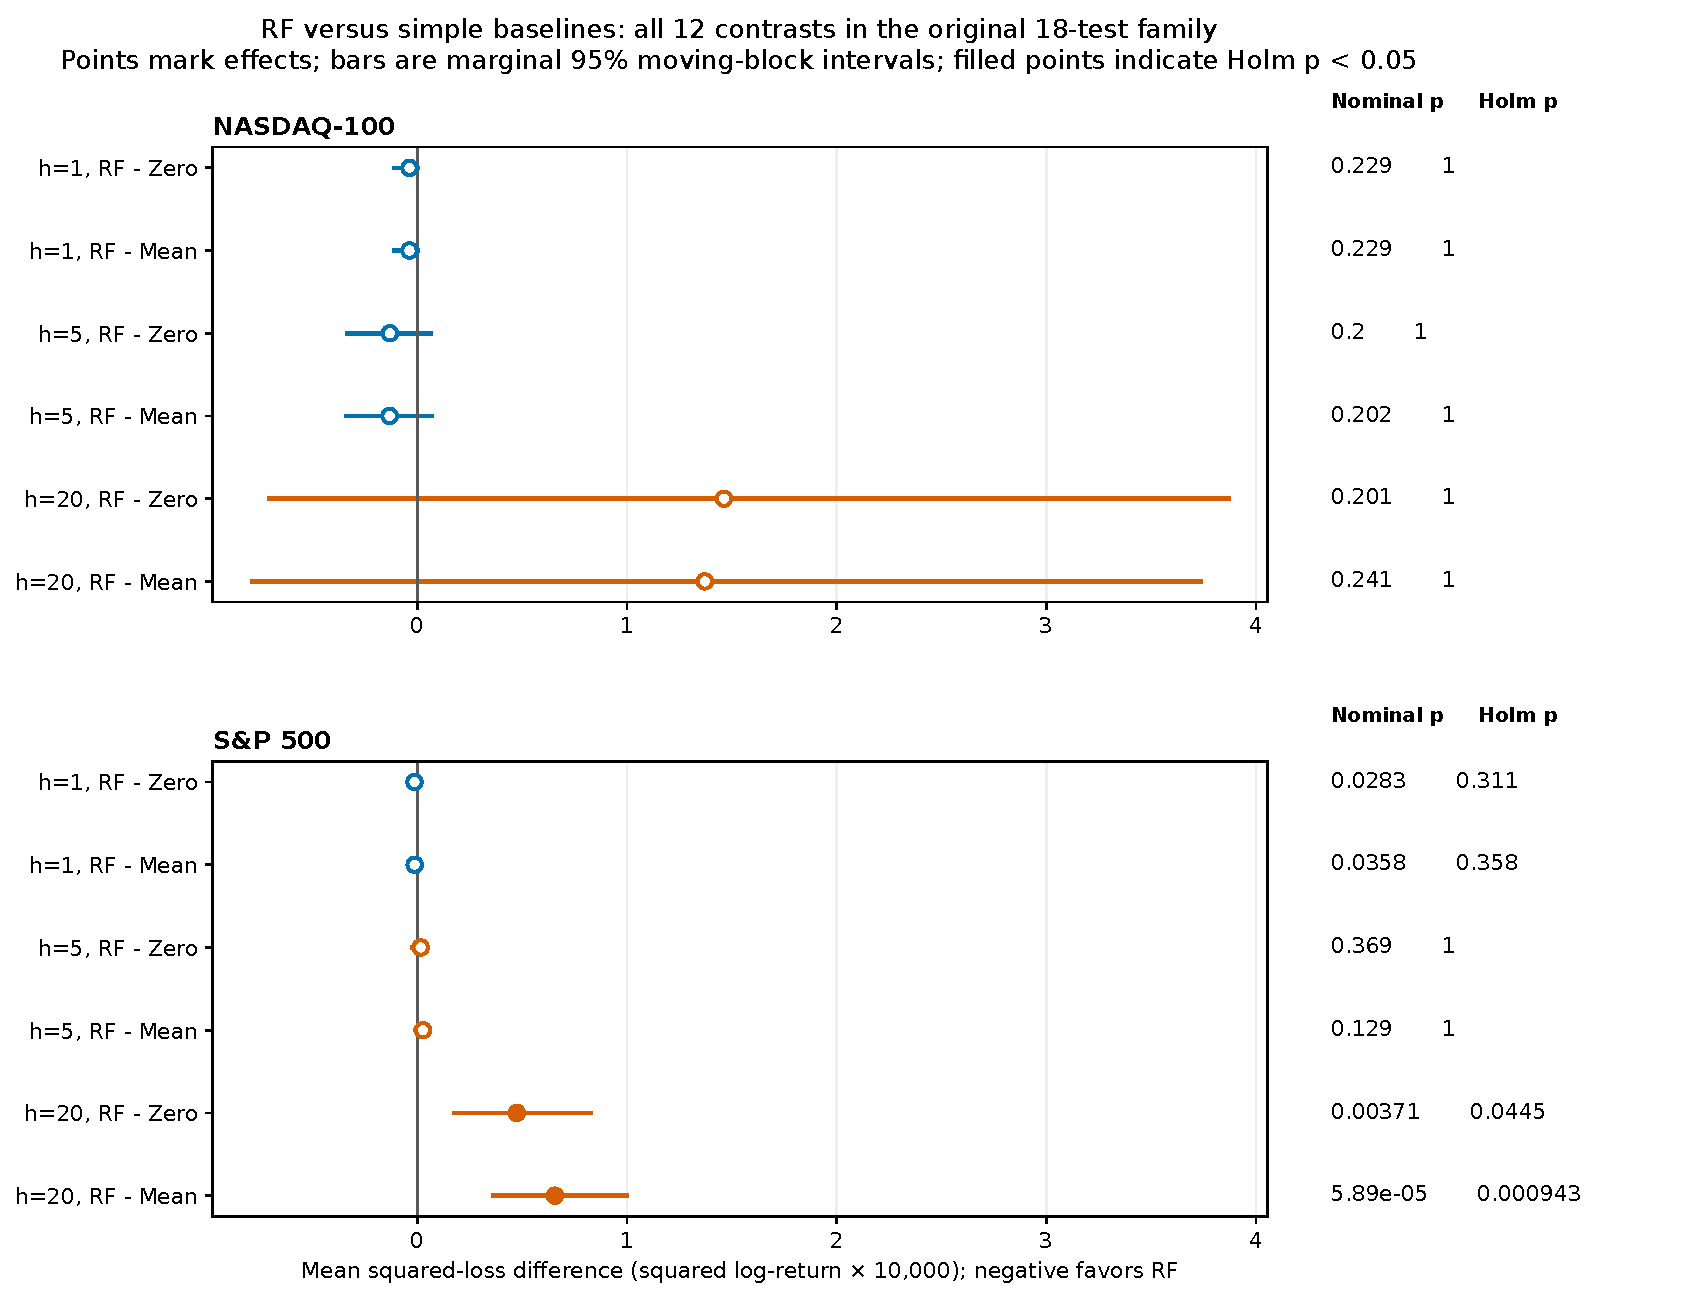
\includegraphics[width=\textwidth]{figures/baseline_effects.pdf}
\caption{All twelve original RF versus simple-baseline contrasts. Bars are marginal 95\% moving-block intervals; nominal and Holm p-values remain separate, with adjustment over the full 18-test family including RF versus LSTM.}
\end{figure}

For NASDAQ h1 RF versus zero, the mean MSE difference is -3.7108856e-06, with marginal interval [-1.0928368e-05, 2.5630173e-07], nominal p=0.22909 and Holm p=1. This illustrates why a favorable pooled skill is not automatically a corrected statistical finding. S\&P h20 RF versus historical mean is unfavorable: difference 6.5652921e-05, interval [3.6398136e-05, 9.999274e-05], nominal p=5.8916e-05 and Holm p=0.000942656. No RF improvement over a simple baseline survives the original correction; RF has adjusted evidence of lower error than LSTM in 5 cells and higher error than the simple baselines in the two S\&P h20 comparisons. Neither observation demonstrates trading value. [C09,C26,C34,C39,C40]

\section*{9. Robustness and sensitivity}

The original seed study selected earliest/middle/latest folds per cell; the expansion added intervening quarter-position folds at the same budgets. Combined sensitivity covers 30 distinct folds and 1260 origins per cell, conditional on the five seeds. The added 60 training runs generated 30240 stochastic forecasts; this is not five-seed replication of all 282 historical folds. Deterministic predictions are reused on the same selected origins rather than represented as independently trained repetitions. [C01,C05,C06,C07,C36,C37]


\Needspace{191pt}
{\footnotesize
\begin{longtable}{llllll}
\caption{Expanded selected-fold stochastic sensitivity: min/max across fixed seeds, not confidence intervals.}\\
\toprule
Index & h & Model & RMSE min & RMSE max & Rank range\\
\midrule\endfirsthead
\toprule
Index & h & Model & RMSE min & RMSE max & Rank range\\
\midrule\endhead
NASDAQ-100 & 1 & RF & 0.011669 & 0.011678 & 1--1\\
NASDAQ-100 & 1 & LSTM & 0.011975 & 0.012151 & 5--5\\
NASDAQ-100 & 5 & RF & 0.024486 & 0.024563 & 1--1\\
NASDAQ-100 & 5 & LSTM & 0.024964 & 0.025514 & 5--5\\
NASDAQ-100 & 20 & RF & 0.044147 & 0.044398 & 2--5\\
NASDAQ-100 & 20 & LSTM & 0.043069 & 0.046180 & 1--5\\
S\&P 500 & 1 & RF & 0.013958 & 0.014012 & 1--1\\
S\&P 500 & 1 & LSTM & 0.014319 & 0.014983 & 4--5\\
S\&P 500 & 5 & RF & 0.030495 & 0.030615 & 4--5\\
S\&P 500 & 5 & LSTM & 0.030225 & 0.030536 & 4--5\\
S\&P 500 & 20 & RF & 0.067252 & 0.067746 & 4--5\\
S\&P 500 & 20 & LSTM & 0.064705 & 0.067994 & 2--5\\
\bottomrule\end{longtable}}

The expanded NASDAQ h20 LSTM ranks remain 1--5; choosing its best seed would hide substantial instability. No expanded ML improvement over either baseline survives the separate Holm family. Seed-averaged loss is a fixed-seed estimand, not a sample of independently realized markets. Every model within a cell has identical origins, endpoints and actual labels. [C08,C12,C33]

Endpoint matching in the full historical study retains 2,232 origins per index/horizon. S\&P h5 then has linear regression as the RMSE winner, unlike its native historical-mean winner. This is evaluation-population sensitivity, not evidence of a changed model or a common training history. The selected seed-study calendars have no shared cross-index endpoints, so a cross-index matched seed result is unavailable. Volatility and stress summaries are descriptive where sample support is limited; complete regime/stress evidence is retained in the repository. [C10,C11,C25,C30,E:regimes]

\begin{figure}[htbp]\centering
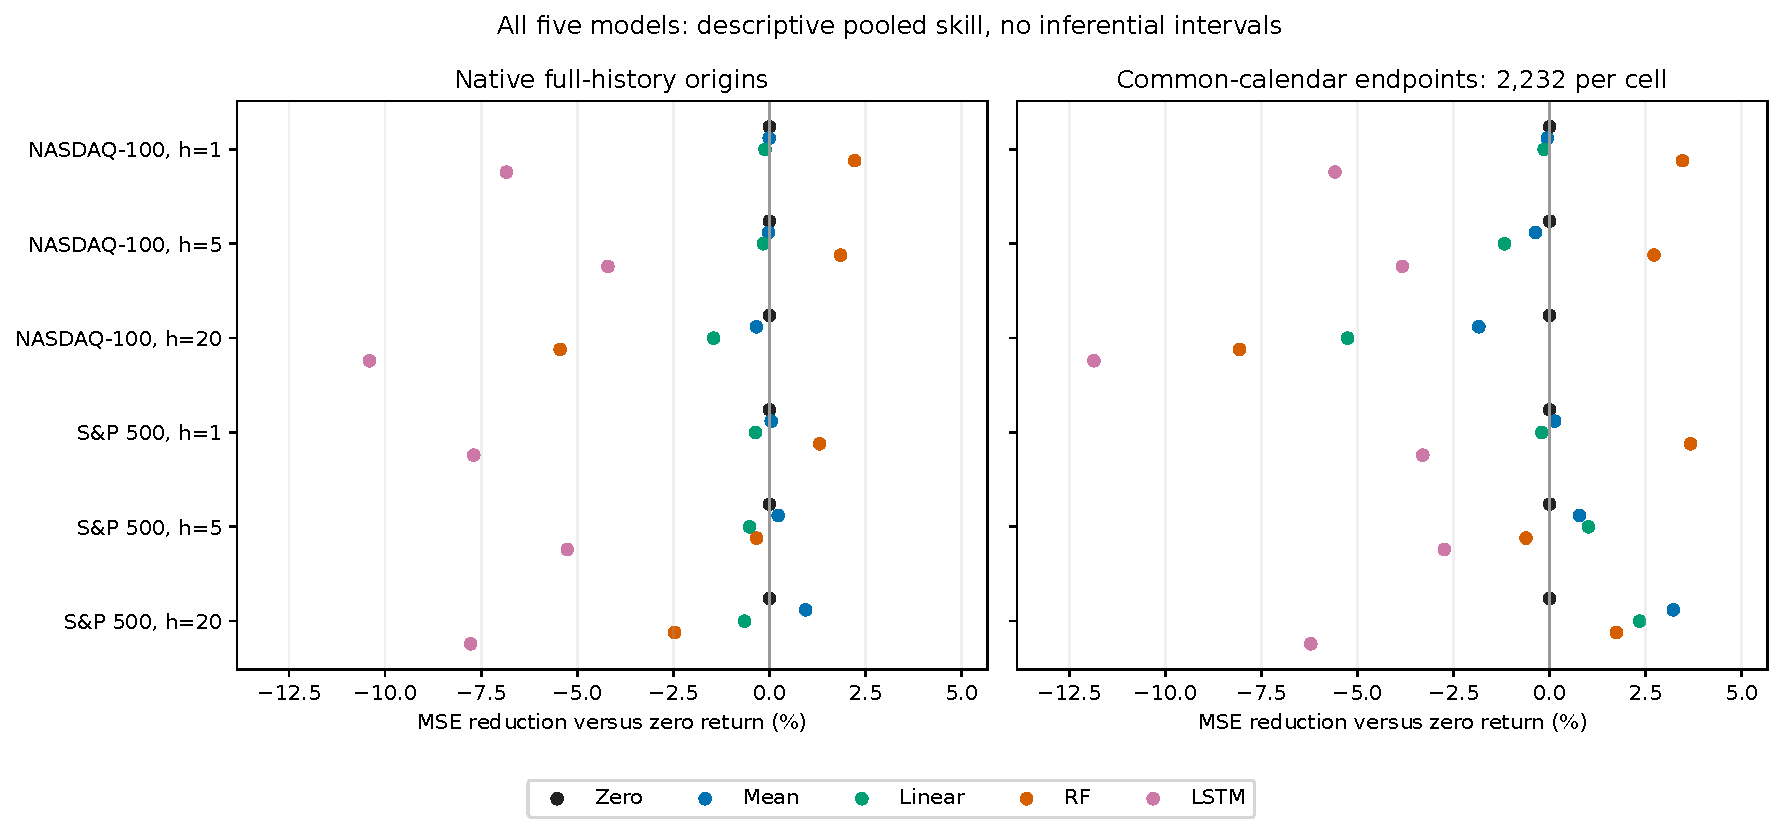
\includegraphics[width=\textwidth]{figures/point_skill.pdf}
\caption{All five point models on native and endpoint-matched populations. MSE skill is relative to zero; these are descriptive points, not confidence intervals.}
\end{figure}

\section*{10. Predictive uncertainty and calibration}

\subsection*{10.1 Fixed prequential intervals}

At origin $t$, a previous residual is usable only if its actual target endpoint date is strictly before $t$. Trailing calibration retains the latest 504 mature absolute residuals, with minimum 252. Expanding calibration uses all mature residuals. Volatility-scaled calibration divides the prior absolute residual by causal volatility at its own origin, then rescales the selected quantile by current causal volatility. The order-statistic rank is $\lceil(n+1)c\rceil$; the public quantile helper returns infinity if that rank exceeds the history rather than silently clipping it. Configured histories make both levels finite. Warmup exclusions remain recorded. [E:calibration,E:protocols]

These intervals calibrate an annually refitted procedure. Earlier OOS outcomes can later enter point-model training. Thus this is not a held-out split-conformal guarantee for one permanently fixed fitted model. All comparisons retain identical eligible origins, and no future realized volatility is used. Nominal coverage is evaluated at 80\% and 90\%, globally and by regime/stress support. [E:calibration,E:tests]

\subsection*{10.2 Delayed adaptive variants}

The adaptive variants use windows 252/504 and update rates 0.01/0.05, with a minimum 252 residuals. Each nominal level has its own state initialized to its target miscoverage. Only a mature, previously eligible interval supplies its own miss indicator $e_i$. The update is $\alpha\leftarrow\mathrm{clip}(\alpha+\gamma((1-c)-e_i),0.02,0.5)$. Warmup forecasts provide residuals but no invented interval feedback. The radius uses rank $\lceil(n+1)(1-\alpha)\rceil$. Clipping and delayed feedback are deliberate differences from theoretical ACI; no arbitrary-dependence or finite-sample guarantee is asserted. [E:adaptive,E:protocols]

The designated sensitivity uses window 504 and rate 0.01; it was not chosen as the winner of the retrospective evaluation. All four variants remain available. The extension stores 1421280 method-origin records and checks 2780000 eligible level/bound pairs. Repeated methods/levels do not create additional independent outcomes. [C13,C14,E:adaptive]

\subsection*{10.3 Coverage, width and interval scores}

Table 4 shows all index/horizon cells for zero-return 90\% intervals under trailing, designated adaptive and volatility scaling. This is a clearly labelled view of the method trade-off, not a restriction of the statistical family to the best-looking point model. Complete files include both levels, all point models, all four adaptive variants and the fixed expanding alternative. [C17,C18,C35]


\Needspace{263pt}
{\footnotesize
\begin{longtable}{lllllll}
\caption{Zero-return 90\% intervals: same eligible origins, coverage fraction and log-return width/score.}\\
\toprule
Index & h & Method & n & Coverage & Width & Score\\
\midrule\endfirsthead
\toprule
Index & h & Method & n & Coverage & Width & Score\\
\midrule\endhead
NASDAQ-100 & 1 & Trailing & 3023 & 0.897453 & 0.039848 & 0.060022\\
NASDAQ-100 & 1 & Adaptive & 3023 & 0.900430 & 0.039829 & 0.057099\\
NASDAQ-100 & 1 & Vol-scaled & 3023 & 0.902415 & 0.041267 & 0.053922\\
NASDAQ-100 & 5 & Trailing & 3019 & 0.894667 & 0.082681 & 0.120230\\
NASDAQ-100 & 5 & Adaptive & 3019 & 0.896986 & 0.083161 & 0.115739\\
NASDAQ-100 & 5 & Vol-scaled & 3019 & 0.897317 & 0.088675 & 0.111598\\
NASDAQ-100 & 20 & Trailing & 3004 & 0.884487 & 0.157120 & 0.224022\\
NASDAQ-100 & 20 & Adaptive & 3004 & 0.883489 & 0.153699 & 0.214307\\
NASDAQ-100 & 20 & Vol-scaled & 3004 & 0.891811 & 0.181810 & 0.224657\\
S\&P 500 & 1 & Trailing & 20159 & 0.893447 & 0.028642 & 0.043455\\
S\&P 500 & 1 & Adaptive & 20159 & 0.896870 & 0.028597 & 0.040732\\
S\&P 500 & 1 & Vol-scaled & 20159 & 0.899945 & 0.030163 & 0.039895\\
S\&P 500 & 5 & Trailing & 20155 & 0.891193 & 0.065366 & 0.094630\\
S\&P 500 & 5 & Adaptive & 20155 & 0.893823 & 0.065518 & 0.089950\\
S\&P 500 & 5 & Vol-scaled & 20155 & 0.900868 & 0.070840 & 0.090837\\
S\&P 500 & 20 & Trailing & 20140 & 0.885353 & 0.130294 & 0.189678\\
S\&P 500 & 20 & Adaptive & 20140 & 0.876663 & 0.129460 & 0.187745\\
S\&P 500 & 20 & Vol-scaled & 20140 & 0.894538 & 0.149298 & 0.192601\\
\bottomrule\end{longtable}}

\begin{figure}[htbp]\centering
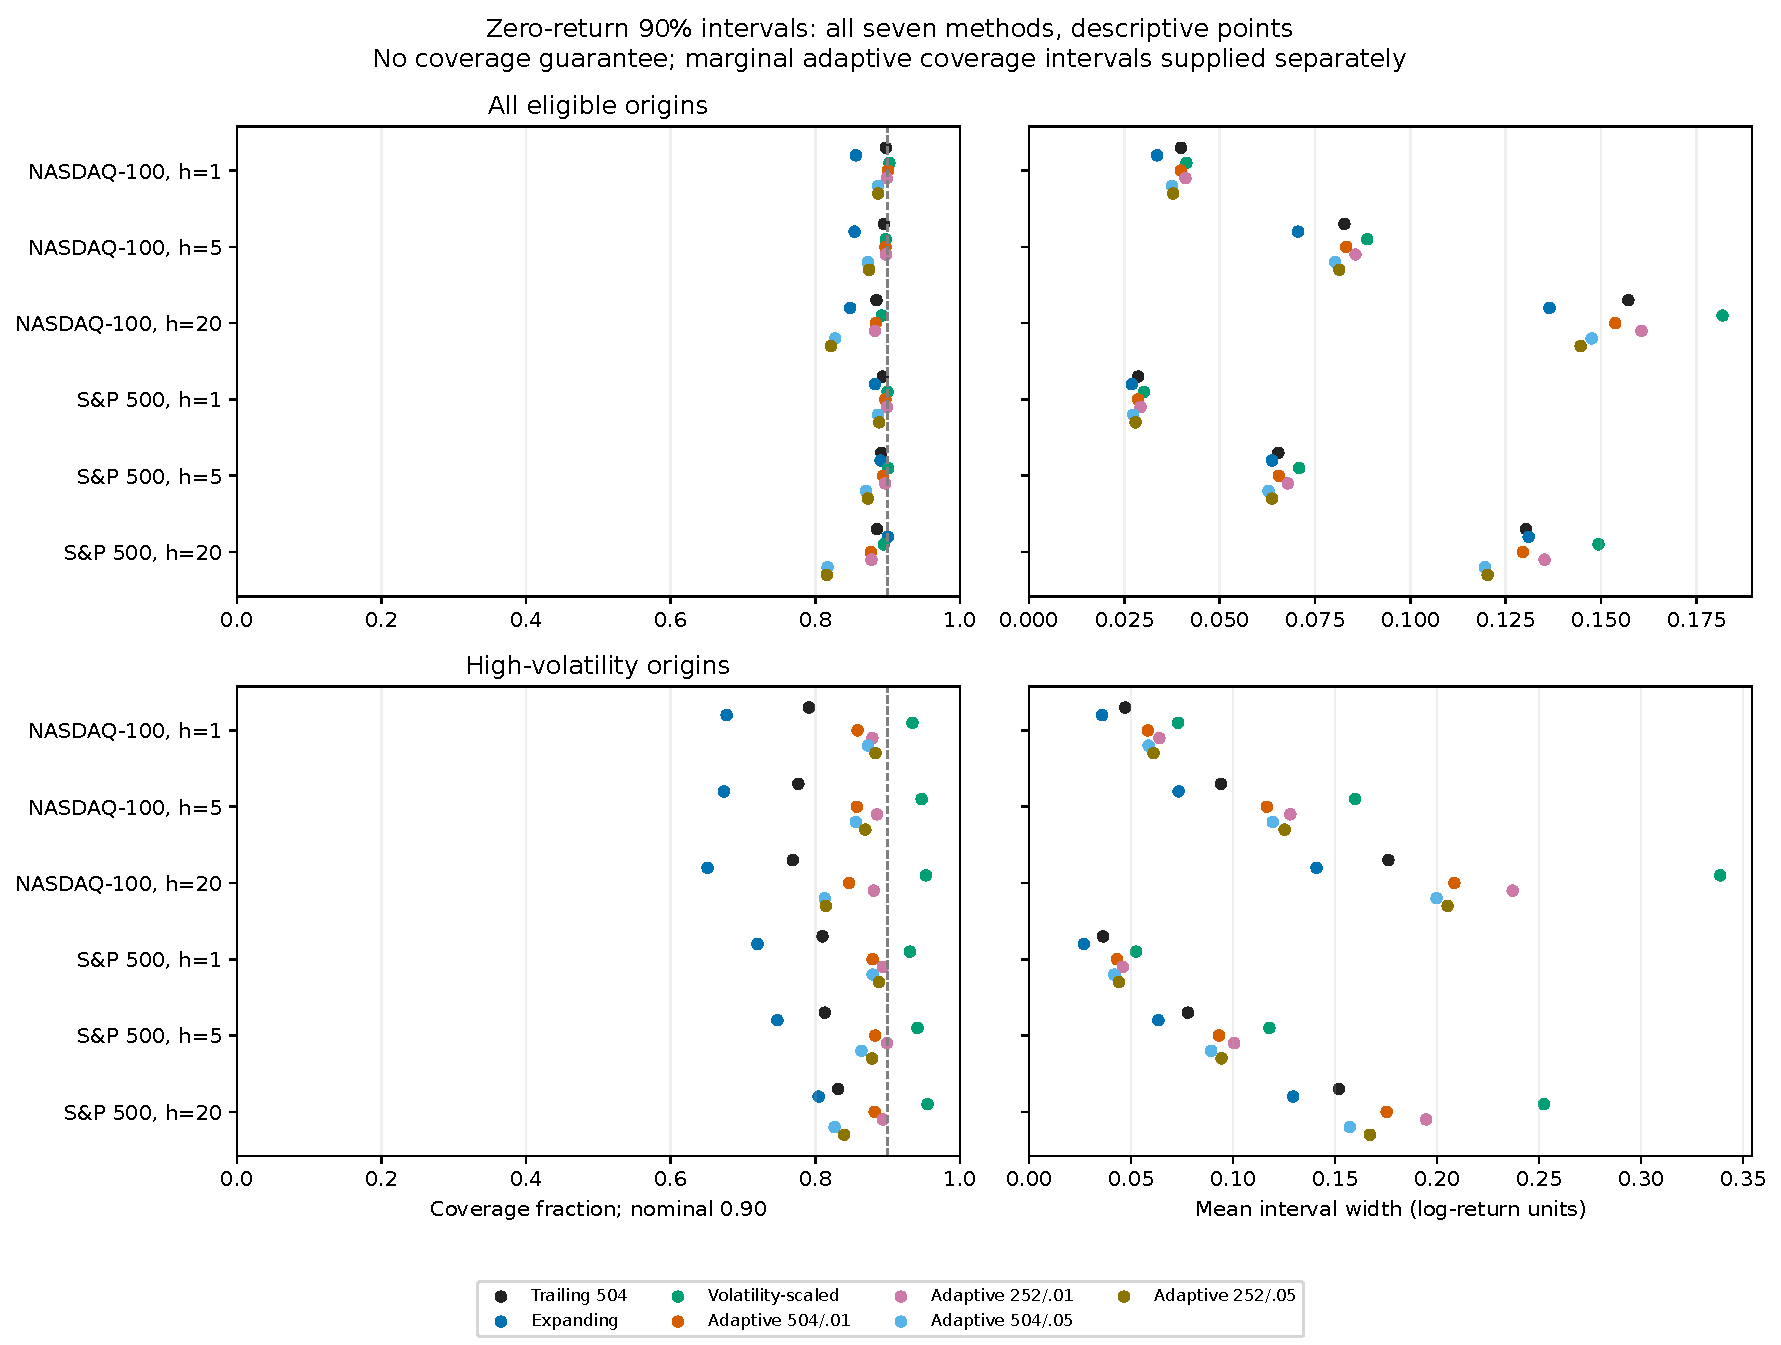
\includegraphics[width=\textwidth]{figures/interval_tradeoffs.pdf}
\caption{Zero-return 90\% intervals for all seven methods, all eligible and high-volatility origins. Points show coverage and log-return width without inferential intervals; adaptive marginal coverage intervals are supplied in the supplementary CSV.}
\end{figure}

The designated variant has 20 adjusted score improvements, all S\&P h1/h5 comparisons across point models and nominal levels. None of its NASDAQ or h20 primary improvements survives correction. For illustration, NASDAQ h1 historical-mean 80\% score improvement has nominal p=0.00685712 but Holm p=0.246856. Selecting only its nominal significance would misstate the result. A small adjusted p-value elsewhere remains retrospective evidence under the inferential approximation, not future calibration assurance. [C15,C16,C35]

For S\&P zero-return h20 90\% intervals, designated adaptive coverage is 0.876663 versus trailing 0.885353, despite a lower mean proper score. NASDAQ h20 high-volatility designated adaptive coverage remains below nominal while volatility scaling covers more broadly with much wider intervals. This documents a trade-off, not a uniformly successful calibration method. [C17]

\subsection*{10.4 Failure cases: clipping and nonnested levels}


\Needspace{95pt}
{\footnotesize
\begin{longtable}{llllll}
\caption{Adaptive failure diagnostics; repeated method-origin pairs and clipped update counts.}\\
\toprule
Window & Rate & Eligible & Crossings & Clipped 80 & Clipped 90\\
\midrule\endfirsthead
\toprule
Window & Rate & Eligible & Crossings & Clipped 80 & Clipped 90\\
\midrule\endhead
252 & .01 & 347500 & 1368 & 1269 & 4070\\
252 & .05 & 347500 & 25819 & 28463 & 19995\\
504 & .01 & 347500 & 1494 & 2114 & 4799\\
504 & .05 & 347500 & 26355 & 30247 & 20876\\
\bottomrule\end{longtable}}

Independent level states can give an 80\% interval wider than its 90\% counterpart. The designated variant has 1494 such violations among 347500 eligible method-origin pairs. Faster variants have substantially more. Counts are accumulated across repeated model procedures and are not independent samples. Alpha clipping is also measured. No hull, monotonic projection or parameter retuning was applied after inspection. Enforcing nesting would define a different method requiring a separately declared evaluation. These experimental variants should not be described as a verified coherent multilevel forecasting system. [C19,C20,C21,C22,C23,E:diagnostics]

\section*{11. Discussion and interpretation}

Three distinctions explain apparent contradictions. First, a local terminal-window winner can differ from a pooled multi-period winner. Second, an adjusted comparison against another complex model does not establish an advantage over a simple baseline. Third, lower proper interval scores can coexist with poorer nominal coverage. Rank changes across seeds or common-calendar populations are empirical instability, not reasons to pick a favorable seed, period or metric. [C07,C10,C11,C17,C24,C26]

Practical relevance requires a decision context. The study does not simulate execution, turnover, costs, risk constraints or portfolio returns. MSE skill and statistical evidence therefore cannot be translated into profitable investment performance. The results also do not prove market efficiency, universal neural-network failure or irrelevance of other features or model families. The defensible conclusion is narrower: these tested procedures do not establish a consistent corrected baseline improvement on the saved evaluation populations.

\section*{12. Threats to validity and limitations}

Researcher selection remains material: the histories were already available, and multiple project stages exposed related outcomes. The declared comparison families constrain individual follow-ups without undoing project-wide exposure. No untouched confirmatory period has been scored. Phase 9's four-block historical rehearsal tests infrastructure only; its model evaluations are not independent chronological validation. The fixed prospective origin and outcome-maturity gates are not a substitute for actually acquired, provenance-reviewed future observations. [C04,C28,C29,E:prospective]

The two dependent US indexes do not constitute independent cross-market replication. Their coverage, construction and training histories differ. The raw files lack complete acquisition versions/timestamps and license provenance. Aggregate index closes do not identify constituent survivorship or dividend reinvestment. Early S\&P-labelled values do not establish a modern-index population throughout the full series. Calendar gaps were preserved, not independently matched to every historical exchange closure. [E:data]

Dependence is not exhausted by the tested block lengths: long-memory dynamics, structural changes and repeated estimation can invalidate normal-reference and bootstrap approximations. Short crisis episodes provide few effective observations, while unavailable NASDAQ episodes cannot support claims. Seed replication covers selected folds; training budgets and candidate grids are limited. There is one canonical recurrent architecture, not a comprehensive neural benchmark. [E:statistics,C07,E:regimes]

The 210 recovered legacy folds have validated records but lack original generating revisions, environments and runtimes. A recovery-time hash is not original acquisition or execution metadata. Model weights are not serialized, and targeted numerical reproduction cannot prove the exact historical training process or platform-independent equality. Original notebook follow-up files are also missing. We preserve these distinctions instead of claiming complete raw-acquisition-to-weight replay. [C03,E:history]

The manuscript and its claim audit are generated from saved evidence and checked computationally within the same workflow. This is not blinded external human peer review. Formal external scrutiny and author/submission decisions remain necessary before a journal or conference submission.

\section*{13. Conclusions and future work}

Under the tested retrospective protocol, model complexity does not establish reliable superiority over simple return baselines. Random-forest point wins are conditional on horizon and population; LSTM pooled errors and seed instability caution against selecting attractive local results. Adaptive score improvements are limited to specified comparisons and coexist with undercoverage, clipping and nonnested intervals. Null findings do not establish equivalence or universal inferiority. [C08,C09,C10,C12,C15,C19,C24]

Future work should execute the frozen prospective protocol only after enough complete, unexposed observations and actual target outcomes exist; acquire additional markets with verifiable source/version/license records; preserve fitted weights and explicit software defaults; and separately predeclare any revised interval-nesting or dependence method. Economic evaluation would require its own decision loss, execution assumptions and costs. These are unresolved research tasks, not experiments claimed to have run.

\section*{Acknowledgments and contribution scope}

The original course project included NASDAQ work by Yug More and S\&P work by Srihan Cheemangunta. This acknowledges the recorded historical contributions and does not presume final manuscript coauthorship or submission consent. No current institutional affiliation or funding relationship is inferred. [E:history]

\bibliographystyle{plainnat}
\bibliography{references}
\section*{Reproducibility appendix}

All displayed numeric precision is presentation rounding of saved values; source CSVs and the machine-readable audit retain the underlying values. Claims C01--C40 resolve to the frozen Phase 12 registry and its source SHA256s. E identifiers resolve to code, configuration and provenance files in \path{paper/evidence/manuscript_manifest.json}. Table sources and selected rows are recorded with the manuscript. These mappings establish traceability; separate recomputation audits establish arithmetic consistency. [E:manuscript]

The required baseline checks are:

\begin{verbatim}
.venv/bin/python scripts/final_synthesis.py verify
.venv/bin/python scripts/audit_all_research.py \
  --output /tmp/marketpulse-audit-new
.venv/bin/python scripts/manuscript.py verify
\end{verbatim}

Use a new output directory for each comprehensive audit because published logs are preserved. An existing directory causes a deliberate refusal rather than replacement. Original fold CSVs can be restored from the committed archive. Expensive refitting is distinct from reconstruction of saved forecast metrics and must not overwrite the original run. Environment metadata, fixed seeds and input hashes support partial numerical reproduction; missing source acquisition records, historical runtime context and unsaved weights limit full replay. [E:history,E:manuscript]

The LaTeX source uses the verified BibTeX entries and a standard compiler. PDF build success, renderer/text-extraction checks, regeneration commands and environment limitations are recorded separately. A passing source checksum alone does not establish visual layout quality or external scientific validity. The reproduction guide and later scientific verification report should be read together with the paper.
\end{document}
